\documentclass{article}
\usepackage[magyar]{babel}
\usepackage{lipsum}
\usepackage{t1enc}
\usepackage{graphicx}
\usepackage{subcaption}
\usepackage{array}
\usepackage{xcolor}
\usepackage[table,xcdraw]{xcolor}
\usepackage{multirow}
\usepackage{wrapfig}
\usepackage{listings}
\usepackage{float}

\frenchspacing % Francia spacing szabályok alkalmazása

\lstset { % A listings csomag beállításai
    language=Python,
    basicstyle=\ttfamily\small,
    frame=single,
    numbers=left,
    numberstyle=\tiny\color{gray},
    stepnumber=4,
    numbersep=10pt,
    tabsize=2,
    showstringspaces=false,
    linewidth=\textwidth,
    framextopmargin=10pt,
    framexleftmargin=15pt,
    framexrightmargin=10pt,
    backgroundcolor=\color{white}
    keywordstyle=\color{blue},
    commentstyle=\color{green},
    stringstyle=\color{red},
    escapeinside={\%*}{*)}
}
\lstdefinestyle{cstyle} {
	backgroundcolor=\color{gray!30},
	keywordstyle=\color{red!80!red},
    identifierstyle=\color{blue!80!black},
    commentstyle=\color{gray},
    stringstyle=\color{blue},
    breaklines=true,
    numbers=left,
    numberstyle=\tiny\color{gray},
    stepnumber=1,
    numbersep=5pt,
    tabsize=4,
    showstringspaces=false,
    frame=none
}

\floatstyle{ruled}
\newfloat{python}{htbp}{lop}[section]
\newfloat{c}{htbp}{lop}[section]

\begin{document}
\section{Képek}
\listoffigures % Képek listája
\listoftables % Táblázatok listája

% Illesszünk be egy képet max. 5cm-es szélességgel, magassággal, torzítás nélkül:
\begin{figure}
	\centering
	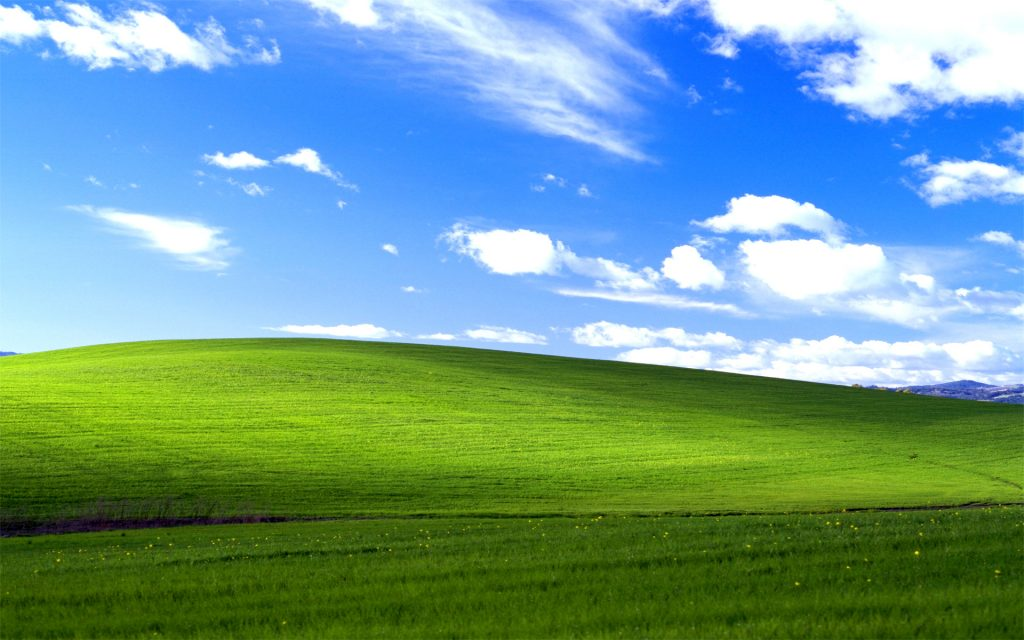
\includegraphics[width=5cm, height=5cm, keepaspectratio]{szines.jpg}
	\caption{Az első ábra}
\end{figure}

A kép maradjon úsztatás nélkül, a szöveggel egy sorban. Előte és utána is generáljuk egy-két bekezdés "zagyva" szöveget:\\\\
\lipsum[1]
\noindent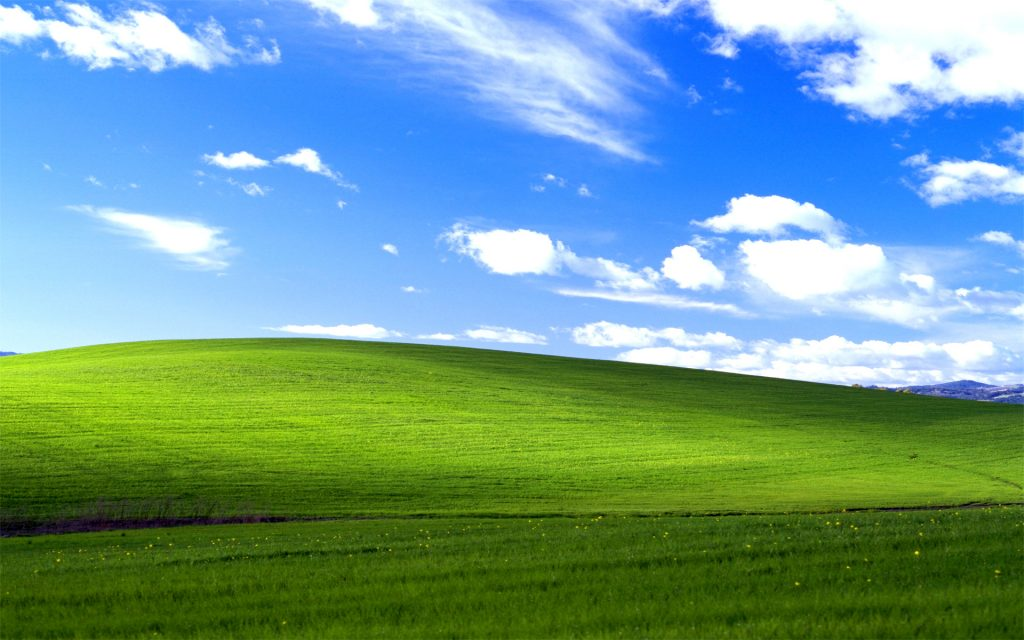
\includegraphics[width=5cm, height=5cm, keepaspectratio]{szines.jpg}\hfill
\lipsum[2]\\

Illesszünk be egy másik képet és helyezzük az úszó ábra környezetébe, és pluszban egy másik kép, valamilyen transzformációval:\\
\begin{figure}[htbp]
	\centering
	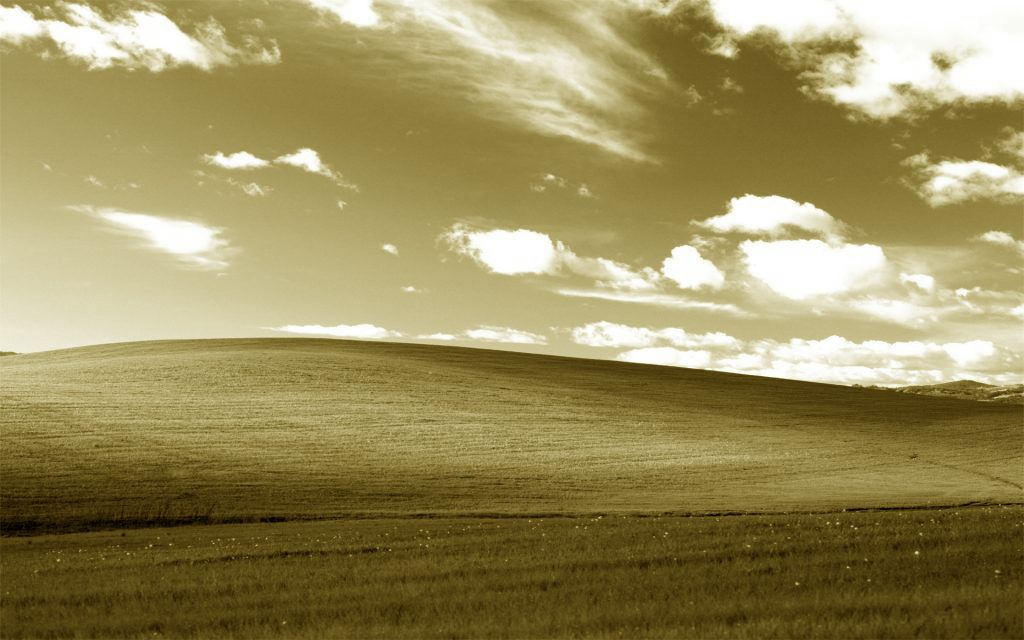
\includegraphics[width=5cm, height=5cm, keepaspectratio]{szepia.jpg}
	\caption{Ez egy úszó ábra}
\end{figure}

\begin{figure}[htbp]
	\centering
	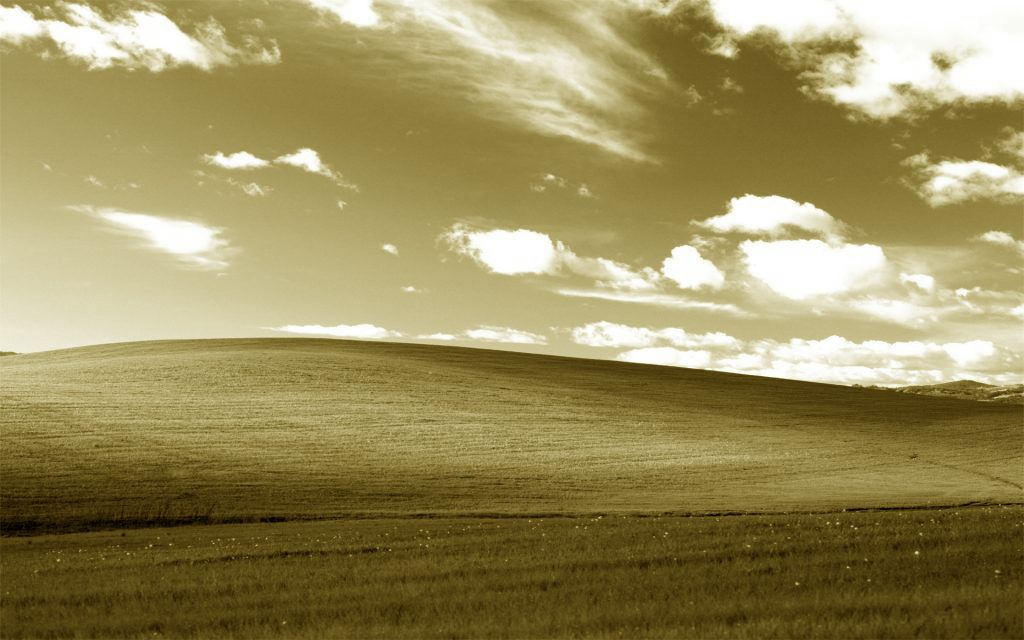
\includegraphics[width=5cm, height=5cm, angle=180, keepaspectratio]{szepia.jpg}
	\caption{Ez egy transzformált úszó ábra}
\end{figure}

\textbf{Lefordul, de "Hibásan", és +1 számozással mutat egy nem létező ábrára.}

Az ábra környezeten belül, hozzunk létre részábra környezetet mindkét képnek:\\
\begin{figure}
	\centering
	\begin{subfigure}[b]{0.45\textwidth}
		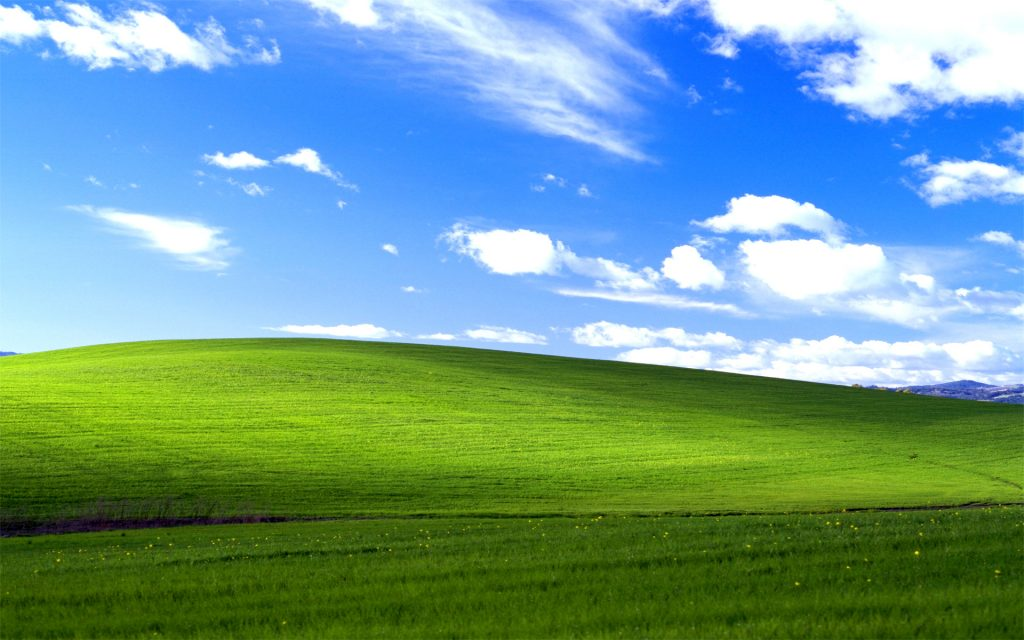
\includegraphics[width=5cm, height=5cm, keepaspectratio]{szines.jpg}
		\caption{Első részábra.}
	\end{subfigure}
	\hfill
	\begin{subfigure}[b]{0.45\textwidth}
		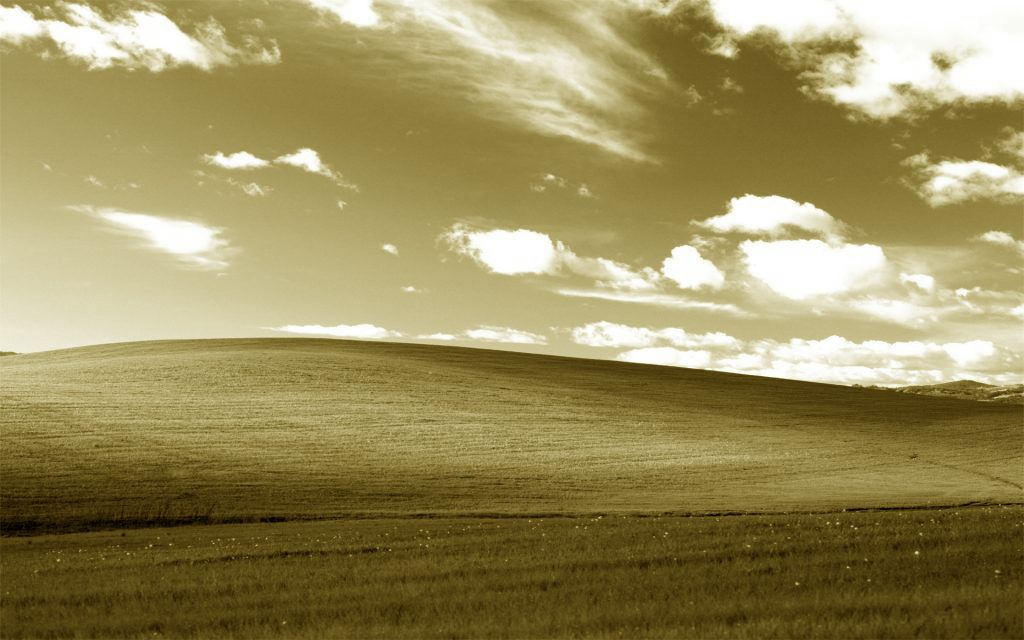
\includegraphics[width=5cm, height=5cm, keepaspectratio]{szepia.jpg}
		\caption{Második részábra.}
	\end{subfigure}
	\vfill
	\caption{Két részábra egymás mellett.}
\end{figure}

\section{Táblázatok}
\begin{table}
\centering
\begin{tabular}{|>{\raggedright\arraybackslash}p{30pt}|c|>{\raggedleft\arraybackslash}p{30pt}|}
\hline
\textbf{Első oszlop} & \textbf{Második oszlop} & \textbf{Harmadik oszlop}\\
\hline
\hline
Szöveg 1 & Szöveg 2 & szöveg 3 \\
\cline{1-3}
& Szöveg 5 & Szöveg 6 \\
\cline{2-3}
Szöveg 7 & & Szöveg 9 \\
\hline
\end{tabular}

\caption{Egyszerű táblázat.}
\end{table}

% 2. táblázat
\begin{table}[h]
\centering
\arrayrulecolor{green}
\begin{tabular}{>{\columncolor{gray}\color{white}}p{30pt}|c>{\raggedleft\arraybackslash}p{40pt}}
\color{green} egy & kettő & három \\ \hline
négy & öt & hat \\
hét & nyolc & \cellcolor{green} kilenc \\
tíz & tizenegy & tizenkettő \\
\end{tabular}
\caption{Színes táblázat.}
\end{table}

\clearpage
% 3. táblázat
\begin{wraptable}{l}{4cm}
\arrayrulecolor{black}
\begin{tabular}{|c|cc|}
\hline
egy                   & \multicolumn{2}{c|}{kettő}                  \\ \hline
\multirow{2}{*}{négy} & \multicolumn{1}{c|}{öt}        & hat        \\ \cline{2-3} 
                      & \multicolumn{2}{c|}{\multirow{2}{*}{nyolc}} \\ \cline{1-1}
tíz                   & \multicolumn{2}{c|}{}                       \\ \hline
\end{tabular}

\caption{Táblázat úszó környezetben, egybevont cellákkal.}
\end{wraptable}

\clearpage
\section{Verbatim}
Ez itt egy példa mondat, amiben inline \verb|\textbf{szöveg}| parancsokat használok.

\section{Programkód 1}
\begin{python}
	\caption{bináris keresés}
	\lstinputlisting[language=Python] {bin_ker.py}
\end{python}

\clearpage
\section{Programkód 2}
\begin{c}
	\caption{bináris keresés}
	\lstinputlisting[language=C, style=cstyle, firstline=4, lastline=14] {bin_ker.c}
\end{c}

\begin{c}
	\caption{rekurzív bináris keresés}
	\lstinputlisting[language=C, style=cstyle, firstline=16, lastline=29] {bin_ker.c}
\end{c}

\end{document}